%%=====================================================================================
%%
%%       Filename:  solution_l4_q456.tex
%%
%%    Description:  Solution to problems 4, 5 and 6 (lecture 4).
%%
%%        Version:  1.0
%%        Created:  03/10/2017
%%       Revision:  none
%%
%%         Author:  Dilawar Singh (), dilawars@ncbs.res.in
%%   Organization:  NCBS Bangalore
%%      Copyright:  Copyright (c) 2017, Dilawar Singh
%%
%%          Notes:  
%%                
%%=====================================================================================

\documentclass[a4paper,10pt]{article}
\usepackage{pgf,tikz}
\usepackage{pgfplots}
\usepackage{amsmath}
\usepackage{amssymb}
\usepackage{siunitx}
\usetikzlibrary{shapes,backgrounds,decorations,decorations.pathmorphing}
\usetikzlibrary{external}
\usetikzlibrary{shapes,shadows,circuits.ee.IEC}
\tikzexternalize 

% Title Page
\title{Lecture 3, Problems 2,3,4,5,and 6} 
\author{Dilawar Singh}
\date{\today}
\begin{document}

\maketitle

\paragraph{Problem 2 - 5 Points}
I want to record from a neuron. The voltage output of the neuron is in the range
-80 to +20 mV. Why can’t I just measure it by directly connecting the electrode
to the oscilloscope?

\paragraph{Solution} An ideal instrument - especially the one which is used to
measure very small signals - must not load the input source; for example, if I
use a measure temperature fluctuation in a cell using a sensitive thermometer
which makes contact with the cell, I may not be able to. Because most of heat is
likely to be lost in the cell-thermometer junction or in thermometer metal head.
Similarly when we use oscilloscope to measure very 'weak' signal, we make sure
that oscilloscope does not consume a significant part of signal itself. The
measure of how effective an instrument is for measuring weak electrical signal
is 'input resistance'. Higher the input resistance, lesser the current flows
into the oscilloscope. 

Enough talk. Let do some number crunching. Lets use a compartment model of
neuron and measure the voltage using 3 different oscilloscope. First, with an
oscilloscope of \SI{1}{\mega \ohm} resistance, then with an oscilloscope with
\SI{10}{\mega \ohm} resistance, and finally with an ideal oscilloscope (with infinite input
resistance). 

\par

\begin{tikzpicture}[scale=1]
    \begin{axis}[
    xlabel=Time,ylabel=Volt
    , grid style={draw=gray!20}, grid = both, minor tick num = 4 
    , xmax = 2e-3
    , legend style={at={(1.2,1)}, anchor=north}
    ]
    \addplot [color=blue,thick] gnuplot [ raw gnuplot ] {
        set datafile separator ';';
        plot "./with_input_resistece.csv" using 1:2 with lines
    };
    \addplot [color=black,thick] gnuplot [ raw gnuplot ] {
        set datafile separator ';';
        plot "./with_input_resistece_100M.csv" using 1:2 with lines
    };
    \addplot [color=red,thick] gnuplot [ raw gnuplot ] {
        set datafile separator ';';
        plot "./without_input_resistence.csv" using 1:2 with lines
    };
    \legend{Oscilloscope with 1M $\Omega$ 
    , Oscilloscope with 100 M $\Omega$, Ideal oscilloscope};
    \end{axis}
\end{tikzpicture}

You'll get full credit if your drive this point home; or get closer to this.

\paragraph{Problem 3 - 5 Points}
\label{par:Problem 4}
What would happen if you increased the frequency of square wave current input to 
an equivalent circuit of a neuron? Draw the waveform at 1, 10, 100 and 1000 Hz, 
explaining.

\paragraph{Solution} Let's start with our single compartment neuron (notice that
$R_a$ is not playing any role in this circuit).

\begin{figure}[h]
    \centering
    \begin{tikzpicture}[circuit ee IEC
        ]
        % Connect R_a
        \draw (-3,0) to[resistor={info={$R_a$}}] ++(3,0)
        ;
        \draw (0,0) -- ++(0,-0.5) -- ++(-1,0)
        to[resistor={info={$R_m$}}] ++(0,-2) 
        to[voltage source={direction info={<-,volt=0.06}}] ++(0,-1.5)
        ;
        \draw (0,0) -- ++(0,-0.5) -- ++(1,0)
        to[capacitor={info={$C_m$}}] ++(0,-3.5) -- ++(-2,0)
        ;
        \draw (0,-4.0) -- ++(0,-0.5) to[ground] ++(0,-0.5)
        ;
        %% Connect a probe to inject current 
        \draw  (2,1) to[current source={direction info={->,ampere=10p}}] ++(-1,0)
            -- ++(-1,-1) node [above] {$b$}
        ;
        \draw (2,1) -- ++(1,0) to[ground] ++(0.5,0)
        ;

    \end{tikzpicture}
    \caption{Injecting current into cell. Axial resistance $R_a$ is useless now.
    We measure voltage at node $b$ when current is being injected into cell.}
    \label{fig:sphere}
\end{figure}

For some typical values of $R_m$, $C_m$, I solve this circuit and plot the
waveforms for given frequencies. When I plot them together, I see the following:

\def\height{6cm}
\begin{tikzpicture}[scale=1]
    \begin{axis}[
    xlabel=Time,ylabel=Volt
    , grid style={draw=gray!20}, grid = both, minor tick num = 4 
    , height = \height
    ]
    \addplot [color=blue] gnuplot [ raw gnuplot ] {
        plot "./output_1hz.txt" using 2:3 with lines;
    };
    \end{axis}
\end{tikzpicture}
\begin{tikzpicture}[scale=1]
    \begin{axis}[
    xlabel=Time,ylabel=Volt
    , grid style={draw=gray!20}, grid = both, minor tick num = 4 
    , height = \height
    , xmax = 0.2
    ]
    \addplot [color=blue] gnuplot [ raw gnuplot ] {
        plot "./output_10hz.txt" using 2:3 with lines;
    };
    \end{axis}
\end{tikzpicture}

\begin{tikzpicture}[scale=1]
    \begin{axis}[
    xlabel=Time,ylabel=Volt
    , grid style={draw=gray!20}, grid = both, minor tick num = 4 
    , height = \height
    , xmax = 0.06
    ]
    \addplot [color=blue] gnuplot [ raw gnuplot ] {
        set xrange [0:0.1];
        plot "./output_100hz.txt" using 2:3 with lines;
    };
    \end{axis}
\end{tikzpicture}
\begin{tikzpicture}[scale=1]
    \begin{axis}[
    xlabel=Time,ylabel=Volt
    , grid style={draw=gray!20}, grid = both, minor tick num = 4 
    , height = \height
    , xmax = 0.006
    ]
    \addplot [color=blue] gnuplot [ raw gnuplot ] {
        plot "./output_1000hz.txt" using 2:3 with lines;
    };
    \end{axis}
\end{tikzpicture}

You were not suppose to give detailed plots but it should become obvious to me
after seeing your plot that you understand what happens to charging and
discharging behaviour of circuit (neuron) when frequency changes. At high
frequencies, neuron is not fast enough (due to?) to follow the input pulse.

\paragraph{Problem 4 - 3 Points}
Draw the equivalent circuit of a myelinated axon segment.

\usetikzlibrary{shapes,shadows,circuits.ee.IEC}
\tikzsetnextfilename{myl}
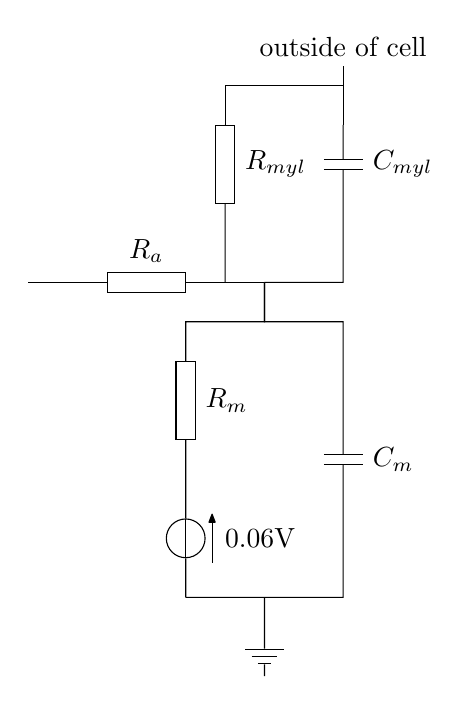
\begin{tikzpicture}[circuit ee IEC ]

    \draw (-0.5,2) to [resistor={info={$R_{myl}$}}] ++(0,-1) -- ++(0,-1);
    \draw (1,2) to [capacitor={info={$C_{myl}$}}] ++(0,-1) -- ++(0, -1)
            -- ++(-1,0);

    \draw (-0.5,2) -- ++(0, 0.5) -- ++(1.5,0) -- ++(0,-0.5);

    \draw (1,2.25) -- ++(0,0.5) node[above] {outside of cell};

    % Connect R_a
    \draw (-3,0) to[resistor={info={$R_a$}}] ++(3,0)
    ;
    \draw (0,0) -- ++(0,-0.5) -- ++(-1,0)
    to[resistor={info={$R_m$}}] ++(0,-2) 
    to[voltage source={direction info={<-,volt=0.06}}] ++(0,-1.5)
    ;
    \draw (0,0) -- ++(0,-0.5) -- ++(1,0)
    to[capacitor={info={$C_m$}}] ++(0,-3.5) -- ++(-2,0)
    ;
    \draw (0,-4.0) -- ++(0,-0.5) to[ground] ++(0,-0.5)
    ;

\end{tikzpicture}

\paragraph{Problem 5 - 3 Points}
A Purkinje neuron with 8 levels of branching obeys Rall’s Law. If the primary
dendrite is 8 microns in diameter, what is the diameter of the final branches?

\paragraph{Solution} If we assume that each branching points, both branches have
the same diameter then we have $d_n^{3/2} = 2 d_{n+1}^{3/2}$ i.e 
$d_{n+1} = \frac{d_n}{2^{2/3}}$. After 8'th level of branching 
$d_8 = \frac{d_0}{{2^{2/3}}^8} = \frac{d_0}{2^{16/3}} = \frac{d_0}{40.31}$.


\paragraph{Problem 6 - 2 Points}
I take 1 micron of dendrite each from the above Purkinje neuron primary
dendrite, and final dendrite. What is the ratio of axial resistances of these
bits of dendrite?

\paragraph{Solution} Remember axial resistance is $r_a = \frac{\rho A}{l}$.
Area $A$ scales with square of diameter therefore 
$\frac{{r_a}_0}{{r_a}_8} = \frac{{d_0}^2}{{d_8}^2} = \sim 40.31 ^ 2 = 1624.9$


\end{document}          

